\section{Design of Cerberus}
\label{Sec:Scheduler}

\begin{figure}[htp]
\centering
        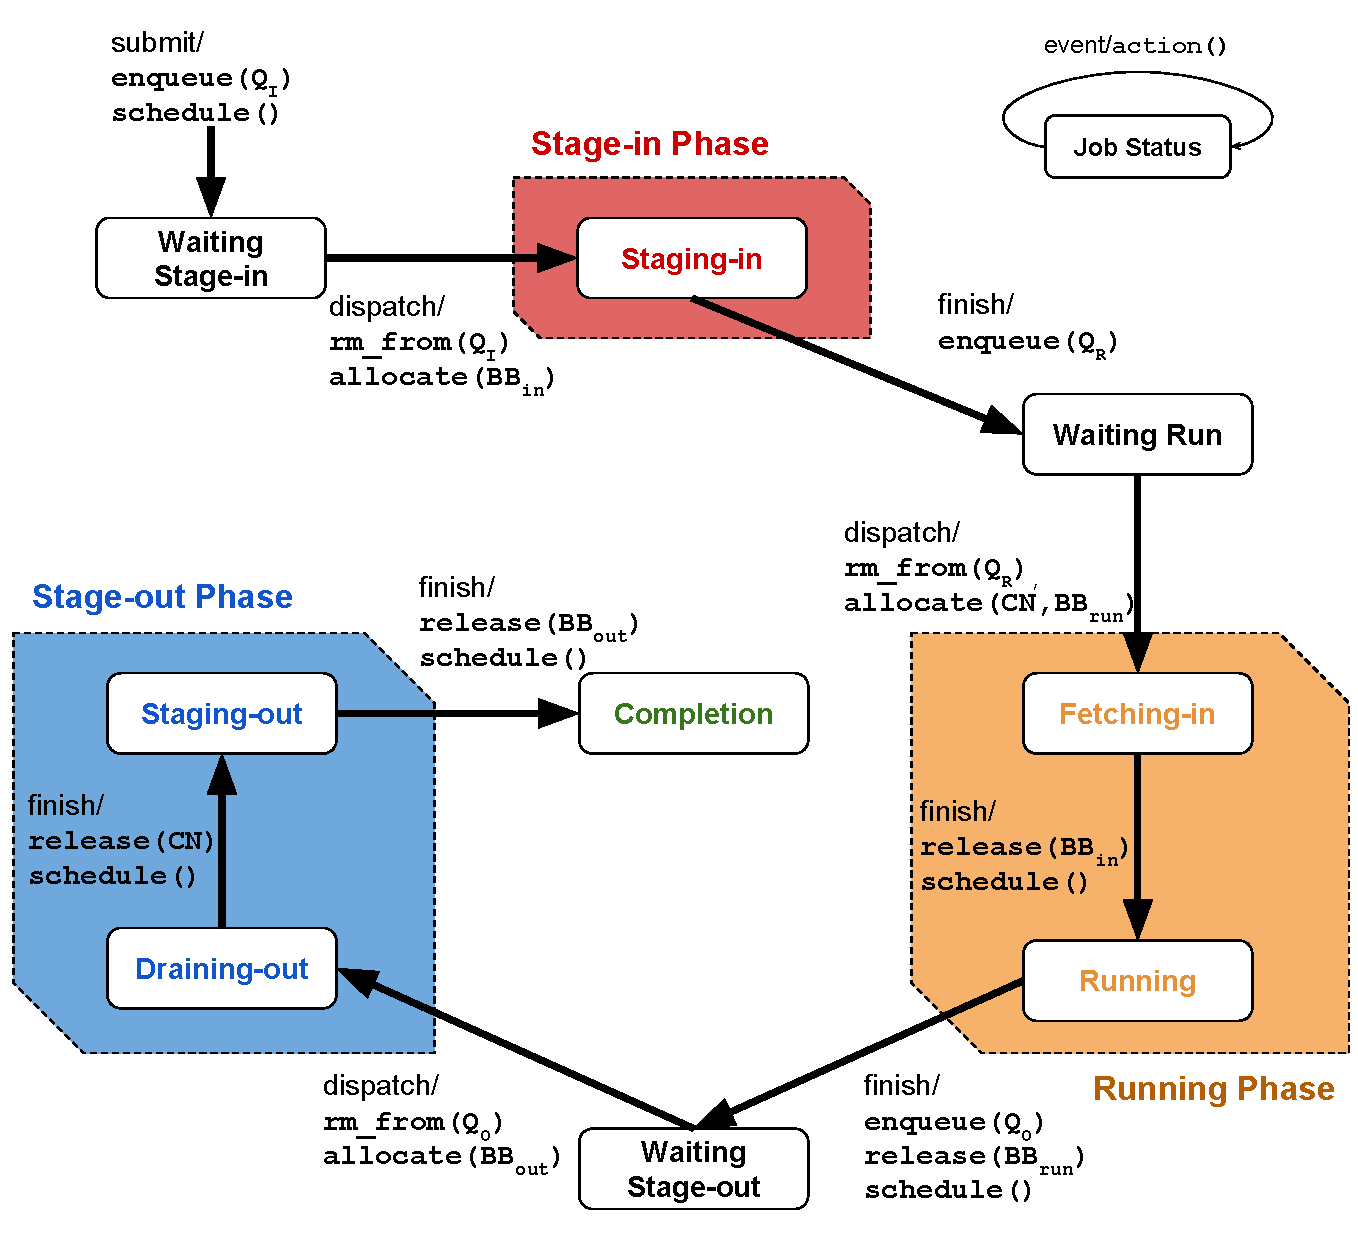
\includegraphics[width=3.6in]{3PhaseJobFSM}
        \caption{Job state transition in Cerberus}
\label{Fig:JobFSM}
\end{figure}

\subsection{Three-Phase Job Scheduling}


%\NOTE{This paragraph moved to start of Section 3}The traditional batch scheduler on a system without burst buffer only considers
%the job with the number of required nodes and the expected runtime for the scheduling decision making process.
%The most commonly used scheduling policy is the First Come First Serve with EASY backfilling~\cite{tsafrir-tpds-2007}.
%However, on burst-buffer-enabled systems,
%the amount of available burst buffer capacity becomes a new scheduling constraint.
%We propose Cerberus, a burst-buffer-aware batch scheduler.
%Cerberus takes the advantage of the most common use cases of burst buffer:
%data stage-in, checkpointing, and data drain-out.
%Cerberus allocates burst buffer in each phase for one of the three use cases
%by maintaining three distinct queues, as shown in Figure~\ref{Fig:CerberusQueues}.
%%Before entering each phase, job must enqueue to the corresponding queue.
%The input queue $Q_I$ contains all the jobs that need to pre-fetch data from the external storage to the burst buffer.
%The running queue $Q_R$ holds the jobs that are waiting for the compute nodes and the burst buffer used for checkpointing.
%Jobs waiting to be drained out to the external permanent storage are in the output queue $Q_O$.
%The layered hierarchy in Figure~\ref{Fig:CerberusQueues} also indicates that burst buffer
%can fill in the memory gap between the memory on compute nodes and the hard disk storage.

As shown in Figure 1, Cerberus adopts a 3-phase job scheduling strategy. 
In order to help understand Cerberus design, we illustrate job state transition in Figure 2.
\TODO{you two should check the paragraph to ensure this part is succinct and precise!--lan\&jin}
To see how Cerberus schedules a particular job with three queues,
we present the job transition diagram in Figure~\ref{Fig:JobFSM}.
After the submission, a job is enqueued into $Q_I$ waiting for the stage-in-purpose burst buffer ($BB_{in}$).
Once selected by Cerberus, the job is removed from $Q_I$ and start to stage in data using the allocated $BB_{in}$.
After finishing the stage-in phase, the job is enqueued to $Q_R$,
where it waits for the compute nodes and the \textit{new} burst buffer for checkpointing ($BB_{run}$).
Note that $BB_{in}$ still holds the job. When Cerberus chooses the job from $Q_R$, the job is in the running phase.
The first thing is to release $BB_{in}$ after \textbf{fetching in} data to memory on the acquired compute nodes.
During the execution, checkpointing and application restart may occur frequently,
which essentially means the data exchanges between the memory and the burst buffer $BB_{run}$.
Once the job execution finishes, $BB_{run}$ can be immediately released since
output data are still available on the compute nodes.
Without releasing the compute nodes, the job enters $Q_O$ and waits for a certain amount of burst buffer for staging out its data ($BB_{out}$).
Once a job is chosen by Cerberus, its data flow from the main memory to the burst buffer
in the \textbf{drain-out} phase, after which all the compute nodes can be released;
then the burst buffer nodes are responsible for transferring the output data to the external storage system.
The job completes when all the useful data results are staged out and $BB_{out}$ are returned to system.
As indicated by Figure~\ref{Fig:JobFSM}, the resource release at anytime can trigger Cerberus
to schedule jobs in multiple queues.

The three-phase job model divides the jobs to generic phases with very specific resource demands.
Cerberus conquers the scheduling problem in each phase, and the detailed decision making is described in Section 4.3 - 4.5.
%The fine scheduling granularity enables the full utilization of burst buffer for different purposes.
%The divide-conquer approach provides a framework that can be extended to various scheduling
%policies for each individual phase.
%We propose and solve two optimizations targeting $Q_I/Q_O$ and $Q_R$ in Section~\ref{Sec:Opt}

\subsection{Three-Phase Coordination}
The three phases together with the corresponding queues, are not entirely independent.
First, only after finishing the stage-in phase can a job be ready for running;
similarly, only when finishing the running phase can a job waiting or entering the stage-out phase.
This is reflected in the lifetime of a job's execution.

Secondly,  the burst buffer demand of any job before entering any phase can only be used for a single purpose.
For example, a running-phase job cannot hold its already taken burst buffer
and to enter stage-out phase upon finishing the running, regardless whether the holding burst buffer has sufficient capacity.
In Cerberus, the resource release is mandatory as specified in Figure~\ref{Fig:JobFSM}.
We believe that frequent releases provide more opportunities to involve the scheduler in each phase for scheduling the jobs.

At last, it is possible that all the three queues are not empty at the moment of scheduling.
We choose a heuristic strategy to determine the scheduling order when
Cerberus has to handle multiple queues at the same time.
Note that jobs finishing the \textit{running} and the \textit{stage-out} phases
will (partially) release the resources, and we set the priority of queues to be $priority(Q_O) > priority(Q_R) > priority(Q_I)$.
This greedy heuristic works well when the demand of the jobs in $J_{Q_I}$ is low.
However, it is possible to make jobs stacking up at the entry of the system.
We plan to investigate this interesting problem in the future.


